\subsection{The Grid Motion Module}

The grid  motion module  smoothly projects deformations  from surfaces
into the  volume mesh.  The algorithm  used by the  grid motion module
employs  an algebraic interpolation  method that  is fast  and robust.
High speed is  obtained through a tree code  acceleration which allows
the interpolation to be evaluated to within a specified accuracy.


\subsubsection{Theoretical Background}
The deformation of the volume mesh can be viewed as a projection of
deformations and rotations from the surface into the volume.  For
general mesh deformations the local surface rotations can estimated
once the displacements are given for each node of the surface mesh.
In the algorithm described in this paper we estimate local rotations
by finding the closest rotation about the node that best matches the
relative displacements of all edges and normals from surface facets
that reference the given node.  Using this information, the
displacement field presented by any surface node can be described as a
rigid body motion.  In our approach, the global deformation field is
given as a weighted sum of these nodal rigid body displacements, where
node $i$ on the deforming surface presents a displacement field,
denoted $\vec{s}_i(\vec{r})$, that is written as
\begin{equation}
\vec{s}_i(\vec{r}) = M_i \vec{r} + \vec{b}_i - \vec{r}, 
\end{equation}
where $M_i$ is a rotation matrix, $\vec{b}_i$ is a displacement
vector associated with the $i^{th}$ node, and $\vec{r}$ is a coordinate
vector in the original mesh.  The displacement field in the volume
mesh is then described through a weighted average of all boundary node
displacement fields as given by
\begin{equation}
\vec{s}(\vec{r}) =\frac{ \sum w_i(\vec{r}) \vec{s}_i(\vec{r})}
    { \sum w_i(\vec{r})}.
\label{eq:deformation}
\end{equation}

For the interpolation weight function, we choose a weighting that is a
function of the reciprocal of distance.  We utilize a two-exponent
form of the weighting function so that we can preserve near-boundary
deformations while providing a smooth transition in the interpolation
to blend deformations in the bulk of the volume mesh.  We also use the
area of the surface facet in the weighting function so that mesh
refinement of a region does not increase its influence in the
interpolation method.  The resulting weighting function is given as
\begin{equation}
w_i(\vec{r}) = A_i * \left[
  \left(\frac{L_{def}}{||\vec{r}-\vec{r}_i||}\right)^a +
  \left(\frac{\alpha L_{def}}{||\vec{r}-\vec{r}_i||}\right)^b \right],
\label{eq:weight}
\end{equation}
where $\vec{r_i}$ is the position of point $i$, $A_i$ is the area
weight assigned to node $i$, $L_{def}$ is an estimated length of the
deformation region, $\alpha$ is an estimated size of the near body
influence region expressed as a fraction of $L_{def}$, and $a$ and $b$
are user-defined exponents.  Numerical experimentation suggests that
$a=3$ and $b=5$ provide the best-quality results.  The $L_{def}$
parameter may be specified by the user, but it is usually determined
automatically by computing the maximum distance any mesh node is from
the mesh centroid.  The alpha parameter controls how much weight is
given to deformations of nearby surfaces relative to more distant
ones.  Generally, this will need to be increased with the variability
in surface displacements.  This appropriate automatic determination of
$\alpha$ can be computed from the deviation of the boundary
displacement field from the mean boundary displacement given by
\begin{equation}
\vec{s}_{mean} = \sum_{i=1}^{N} a_i * \vec{s}_i(\vec{r}_i),
\end{equation}
where $a_i=A_i/\sum_{j=1}^N A_j$ is the normalized node weight and
 $\alpha$ is then determined through the following expression:
\begin{equation}
\alpha = \frac{\eta}{L_{def}}\max_{i=1}^N  ||\vec{s}_i(\vec{r}_i)-\vec{s}_{mean}||.
\label{eq:dynamicalpha}
\end{equation}
The $\eta$ term is a user defined parameter that expresses how far
into the domain a displacement should be ``absorbed.''  Numerical
experiments have found that a value of $\eta=5$ provides satisfactory
results in most cases.  Generally, we limit $\alpha$ to be $0.1$ or
greater to guarantee that a region of rigid deformation is maintained
in boundary layer regions to preserve viscous mesh quality.  This
defines our baseline direct interpolation algorithm.  Our numerical
experiments show that this approach is able to produce high-quality
meshes for large deformations and also is able to preserve mesh
orthogonality near the boundary surfaces.

\subsubsection{Optimizations}

For two-dimensional problems where the number of boundary nodes is
relatively small, the above algorithm runs quite fast.  However, for
three-dimensional problems, the surface nodes grow at a rate of
$O(n^\frac{2}{3})$, where $n$ is the total number of nodes in the
simulation.  Therefore, the cost of the above algorithm becomes
$O(n*n^\frac{2}{3})=O(n^\frac{5}{3})$.  Although the algorithm
parallelizes well, the cost of the deformation calculation quickly
becomes dominant for three-dimensional cases.  However, for mesh
deformation, the accuracy of this evaluation is not critical and only
needs to be accurate to a fairly large fraction of the mesh spacing.
Also, the form of the sum is similar in form to gravitational
potential equations that are solved for N-body simulations.  It is
therefore reasonable to look towards tree-code optimizations similar
to N-body algorithms such as Barnes-Hut\cite{Barnes.1986} and
FMM\cite{Greengard.1987}.  Using these approaches, the cost of the
deformation step could be reduced to $O(n \log n)$, or even $O(n)$ if
suitable kernels for the multipole and local expansions are found.

The Barnes-Hut tree-code algorithm requires that we have an
approximation for the influence of a set of points at some distance
and that we have an estimate for the error in the approximation.  In
the case of N-body simulations, potential theory can be used to
express the influences of a collection of bodies as a multipole
expansion about the centroid.  A truncated expansion can be used to
provide an approximation and also an estimate on error bounds.
Unfortunately, the sums given in equations (\ref{eq:deformation}) and
(\ref{eq:weight}) do not satisfy potential theory and so an analytical
approach to forming a multipole expansion is not readily available.

Lacking this infrastructure, we find an alternative way of
constructing a suitable approximation to the effects of a collection
of particles.  First, we focus on approximating the sum
\begin{equation}
f(\vec{r}) = \sum_{i=1}^N \frac{a_i}{||\vec{r}-\vec{r_i}||^3},
\label{eq:sum}
\end{equation}
where $a_i$ is the normalized node weight.  Instead of attempting to
find a multipole expansion for this sum, we instead focus on finding a
small set of pseudo nodes that can approximate the collection of
particles at a distance, essentially approximating a truncated
multipole expansion.  For example, to approximate a quadripole we
would use four points that share the same centroid as the collection
of points such that our sum is approximated by
\begin{equation}
f(\vec{r}) \approx \frac{1}{4}\left( \frac{1}{||\vec{r}-\vec{q}_1||^3}
+\frac{1}{||\vec{r}-\vec{q}_2||^3}
+\frac{1}{||\vec{r}-\vec{q}_3||^3}
+\frac{1}{||\vec{r}-\vec{q}_4||^3}\right),
\label{eq:approx}
\end{equation}
where $\vec{q}_1,\vec{q}_2,\vec{q}_3,$ and $\vec{q}_4$ represent the
locations of the four approximating pseudo nodes which we call
the quad-points or QPs.  Given the constraint that the QPs share the centroid of the collection given in equation \ref{eq:sum}, we can determine the location of $\vec{q}_4$ using the relation
\begin{equation}
\vec{q}_4 = 4~\left( \sum_{i=1}^N a_i \vec{r_i} \right) - \left( \vec{q}_1 + \vec{q}_2 + \vec{q}_3\right).
\label{eq:centroidconstraint}
\end{equation}

The three remaining QPs are found using a non-linear least squares that minimizes the error given by
\begin{equation}
err  =  ||f(\vec{r})-\frac{1}{4}\left( \frac{1}{||\vec{r}-\vec{q}_1||^3}
+\frac{1}{||\vec{r}-\vec{q}_2||^3}
+\frac{1}{||\vec{r}-\vec{q}_3||^3}
+\frac{1}{||\vec{r}-\vec{q}_4||^3}\right)||^2
\end{equation}
on the test sphere defined by $r=3R_e$ where $R_e$ is the radius of
the smallest centroid centered sphere that contains all of the points,
$\vec{r}_i$.  In our case we minimize the error at the 20 nodes of a
dodecahedron that is circumscribed by the test sphere.  We pick three
points arbitrarily from the collection of points to initialize the
non-linear least squares solve.  An example of this procedure is shown
in figure \ref{fig:QPs} where the small white points show a collection
of 128 random points sampled from the surface of one octant of the
unit sphere.  The dark gray inner region illustrates the enclosing
sphere with radius $R_e$, while the larger sphere illustrates the test
sphere where error is minimized.  The larger blue points show the
location of the computed QPs.  Once we have computed the QP locations,
we utilize 12 additional points on the sphere defined by the centroids
of the dodecahedron faces to sample the errors on the test sphere.
The errors in using the QPs to approximate the sum for both the third
and fifth powers are shown in table \ref{tab:error}.  The table shows
that the approximation error drops as a function of $1/r^2$ for
exponents three and five providing the needed model for approximation
errors.

\begin{figure}
  \begin{center}
    \noindent
    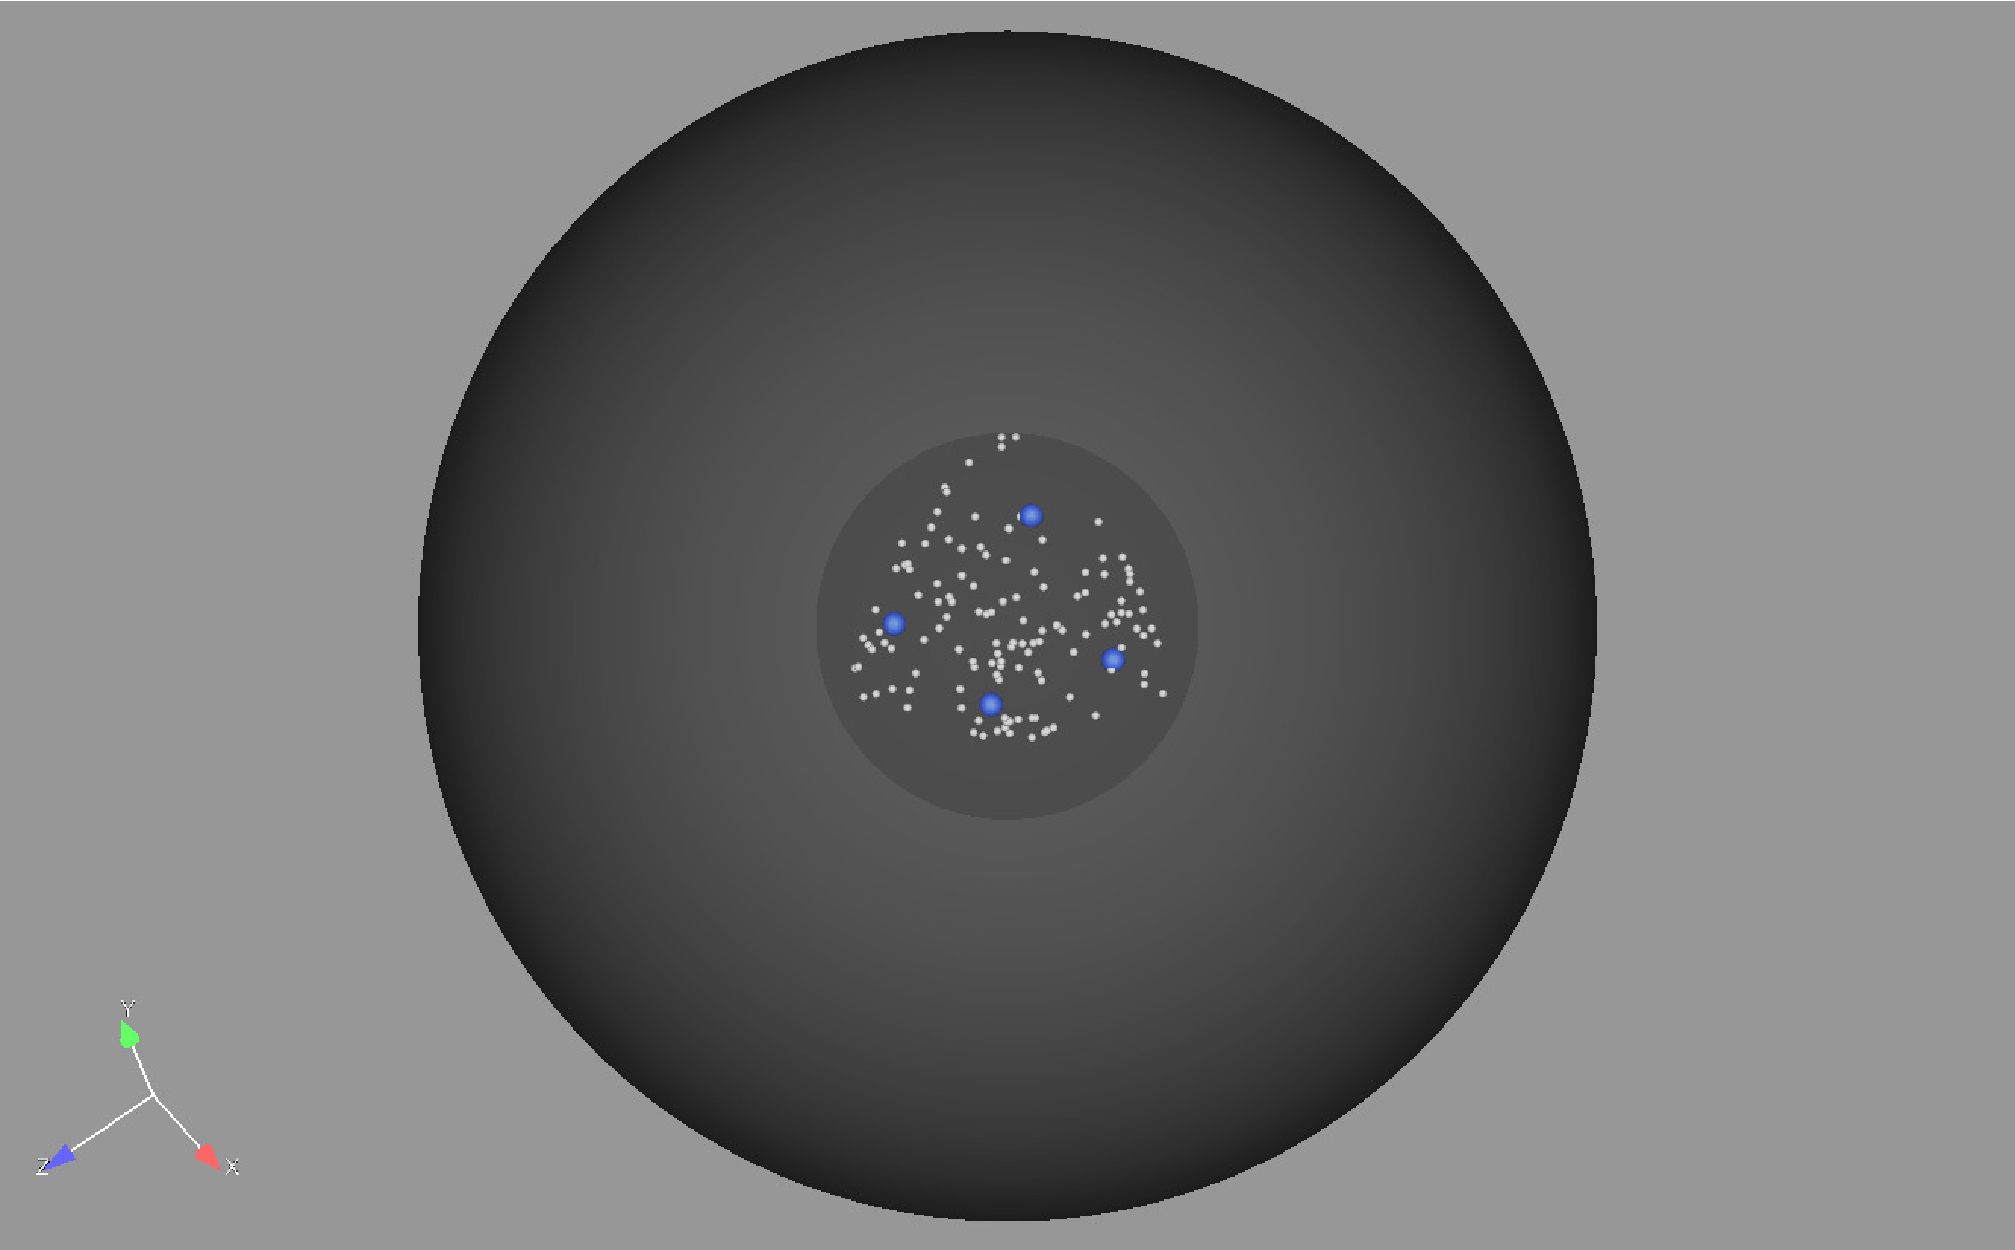
\includegraphics[width=0.75\textwidth]{Figures/points}
  \end{center}
  \protect\caption{Illustration of QP computation}
  \label{fig:QPs}
\end{figure}

\begin{table}[htbp]
\caption{Errors for QP approximation}
\label{tab:error}
\begin{center}
\begin{tabular}{|r||l|l|l|}
\hline
distance  & error         & error \\
(r)       & $(a_i/r_i^3)$  & $(a_i/r_i^5)$ \\
\hline\hline
$3 R_e$   & 0.967\%       & 3.34\%\\
$10 R_e$  & 0.0563\%      & 0.140\%\\
$20 R_e$  & 0.0124\%      & 0.0313\%\\
$40 R_e$  & 0.00290\%     & 0.00737\%\\
$80 R_e$  & 0.000717\%    & 0.00180\%\\
$160 R_e$ & 0.000184\%    & 0.000457\%\\
\hline
\end{tabular}
\end{center}
\end{table}

For general deformations, we also need to consider the implications of
the variation of the rotation matrices, $M_i$, and translation
vectors, $b_i$.  To approximate the effects of these terms, we use the
QPs found in the previous step, but perform a term-by-term least
squares fit in order to assign $M_i$ and $b_i$ to the four
approximation points, again preserving the centroidal value.  The
resulting approximations have similar accuracy profiles to those shown
in table \ref{tab:error}.

\begin{figure}
  \begin{center}
    \noindent
    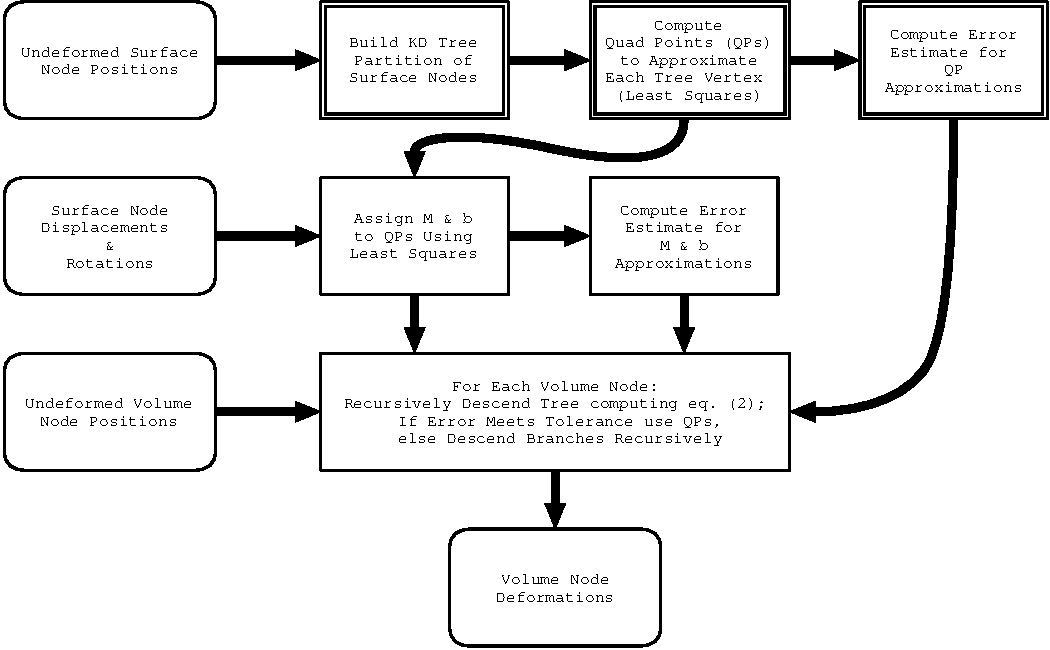
\includegraphics[width=0.75\textwidth]{Figures/fmdmflow}
  \end{center}
  \protect\caption{Mesh Deformation Software Architecture}
  \label{fig:architecture}
\end{figure}

From these approximations, we have the foundation to build a tree-code
fast evaluator.  The architecture of the tree-code mesh deformation
software is shown in figure \ref{fig:architecture}.  The boxes with
double lines only need to be evaluated once using the original
undeformed grids.  The remaining steps, because they depend on the
actual displacements, must be computed every time new displacements are
provided.  The first step is to build the KD-tree to spatially
partition the surface nodes.  To reduce the depth of the tree, we use
bins containing approximately 32 surface nodes for the leaves of the tree.
Once the spatial partition is established we then compute the QPs for
each vertex in the KD-tree.  Once the QPs are determined, the errors
at the test sphere can be measured.  The KD-tree vertices are then
populated with the centroid, containing sphere radius, and measured
errors.  

The final step in the deformation algorithm is evaluating deformations
for the mesh volume nodes (note the deforming surface nodes are
evaluated using the prescribed deformations).  The recursive evaluator
computes the numerator, denominator, and the error in the denominator
of equation (\ref{eq:deformation}).  If we are a leaf of the tree then
the deformation and weights are evaluated exactly forming the base
case of the recursive algorithm.  Otherwise we evaluate the error
associated with using the QP approximation at the current level.  If
the error bound is met, then return the approximate numerator and
denominator, otherwise sum the evaluation of the two children.  Note,
since we compute the accumulated error, there can be an advantage to
evaluating the parts of the tree that give larger weights as this
increases the error threshold for the remaining part of the tree.
Therefore we visit child vertices in the order of closest centroid
first to reduce computational cost.

The behavior of this algorithm automatically reduces errors near the
surface since in this region the nearby leaves will be evaluated as an
exact expansion.  Since the weights associated with these nearby
points will typically be much greater than more distant points, the
error in the boundary layer regions is generally very small regardless
of target error bound.  Further away from the surface we generally
only need the deformation error to be within small fraction of the
edge length.  Typically we find that this requirement is easily met
with a target relative error of just $1\%$.


\subsubsection{Grid Motion User Controls}

The grid motion module is activated by adding an appropriate
{\tt loadModule} command at the top of your vars file:
\begin{verbatim}
loadModule: gridMotion
\end{verbatim}

The global properties of the interpolation can be controlled by user
specified parameters.  In most cases these parameters will work very
well in their default setting, but in specific cases it may be helpful
to make changes.  These controls are represented by the following vars
file variables:

\begin{enumerate}
  \item {\tt gridMotionExpA}
    
    This is the $a$ coefficient described in the weight equation, eq. (\ref{eq:weight}).  This controls how deformations are blended away from the deforming surfaces.  The exponent is a positive integer with a default setting of 3.  A smaller setting will make the blending smoother with a greater risk of having grid line crossing, whereas a larger number will increase shearing in the mesh.  Generally it is good to leave this value as the default.
    
  \item {\tt gridMotionExpB}

    This is the $b$ coefficient described in the weight equation, eq.
    (\ref{eq:weight}).  This controls how deformations are blended for
    points close to the surface.  It is usually set to a larger value
    than $a$ so that the behavior near the body behaves in a more
    rigid manner preserving viscous mesh orthogonality.  The default
    setting for this is 5.

  \item {\tt gridMotionLref}
    
    This is the $L_{def}$ coefficient in the weight equation, eq.
    (\ref{eq:weight}).  This defines the average length over which the
    deformation will be distributed.  If this variable is not set,
    then the deformation length is computed by finding the most
    distant point in the mesh from the mesh centroid.  For many
    problems this is a good default value, but for specific cases,
    particularly where you know the deformation region is much smaller
    than the overall mesh, it may be helpful to set this value to
    something that is sensible to your specific mesh deformation case.

  \item {\tt gridMotionAlpha } 

    This is the $\alpha$ coefficient in the weight equation , eq.
    (\ref{eq:weight}).  This defines the fraction of the deformation
    length that will be reserved for more rigid near-body deformation.
    If this is not set then the value of $\alpha$ will be computed
    dynamically based on equation (\ref{eq:dynamicalpha}).  Usually
    the dynamic alpha provides better results than providing a
    constant value with this setting, so it is advised not to adjust
    this parameter.


  \item {\tt gridMotionAlphaFactor}

    This variable is the $\eta$ parameter in the dynamic alpha
    equation (\ref{eq:dynamicalpha}).  The dynamic alpha will increase
    the stiff region around bodies when they have more complex
    deformations.  The default value is set to 5 which appears to be
    sufficient for most applications.

  \item {\tt gridMotionAlphaFloor}

    This variable sets the minimum value for $\alpha$ that will be
    used when the dynamic alpha computation is being used.  This
    provides a guarantee that near wall regions will remain rigid and
    orthogonal.  The default setting for this value is 0.1.


  \item {\tt gridMoveErrorTol}

    This variable sets the error tolerance of the approximation
    algorithm.  It is a percentage of the minimum edge length attached
    to the node.  The default value is 0.1 which is usually sufficient
    for most applications.  A larger value will degrade mesh quality
    but may improve speed, while a smaller value can improve mesh
    quality if approximation errors were the cause.  Generally this
    value does not need to be changed from the default setting.

  \item {\tt gridDeformationSymmetry}

    This variable is set if you have a symmetry plane at $x=0$, $y=0$,
    or $z=0$.  It is set to the string ``x'', ``y'', or ``z''
    respectively to support the symmetry plane motion.  When using a
    symmetry plane, the plane itself will be allowed to float and the
    deformations will be reflected so that the interpolation at the
    symmetry plane does not include out of plane deflections.

  \item {\tt gridDeformationPlane}

    This variable is set for 2-D simulations to prevent deformations
    in the extruded direction.  It is set to a string specifying the
    extruded axis.

\end{enumerate}

In addition to the global parameters described earlier there are controls that can be provided on a per boundary basis.  Note, if any boundary is not marked with a descriptor for mesh motion, then those nodes will be deformed just as the interior nodes are deformed.  The boundary condition settings for the grid mover are as follows:
\begin{enumerate}
  \item {\tt fixed}

    This setting tells the grid mover that this surface is not moving
    and so the deformation is identically zero for these nodes.

  \item {\tt moving}

    This setting tells the grid mover that this surface will be
    receiving displacements from another module and as such the
    surface will be moving.

  \item {\tt constrainedMotion}

    This setting tells the grid mover that the nodes on this surface
    will be allowed to move but that they are constrained to move
    within a specified surface.  The specified surface can be a plane,
    infinite cylinder, or a discrete geometry file.  Constrained
    motion surfaces are used to interface between moving surfaces and
    fixed surfaces.  Examples of setting a plane constrained motion boundary would which constrains to the plane $x=0$ defined using a point and normal would follow an input such as:
\begin{verbatim}
    back=viscousWall(adiabatic,constrainedMotion=
                     plane(point=[0,0,0],normal=[1,0,0])),
\end{verbatim}
    A cylinder is  similarly defined using a cylinder key word given two points on the cylinder axis and the radius, which would be defined using an input similar to:
\begin{verbatim}
    case=viscousWall(adiabatic,constrainedMotion=
                     cylinder(p1=[0,0,0],p2=[4,0,0],radius=.5)),
\end{verbatim}
    Finally a general geometry constraint can be specified using a geometry file using a {\tt geoFile} keyword such as:
\begin{verbatim}
    case=viscousWall(adiabatic,
                     constrainedMotion=geoFile(file="case.geom")),
\end{verbatim}
    The constrained motion option also allows intersecting constrained surfaces in which case the points that share both surfaces will be constrained to move along the curve of intersection.

  \item {\tt deformWeight}
    
    By default, each node is assigned a weight proportional to its
    local area which means that a large surface may have undue
    influence over the deformation of grid nodes around a nearby
    smaller surface.  The {\tt deformWeight} can be added to a
    boundary to increase (if greater than 1) or decrease (if less than
    1) the influence of that boundary surface on the volume
    deformation.

  \item {\tt farfieldDeform}

    Since farfield boundaries usually have very large areas compared
    to the interior surfaces it is often helpful to mark the farfield
    boundaries with the {\tt farfieldDeform} flag.  This flag will
    automatically provide a {\tt deformWeight} to the farfield
    boundaries that is formed by the ratio of the all non-farfield
    boundaries to the farfield area.  This will reduce the influence
    of the farfield on the volume deformation.

\end{enumerate}
